\documentclass{article}

\usepackage{shared}

\usepackage{biblatex}
\addbibresource{references.bib}

\title{SCARV: RISC-V Crypto ISE \\ Reference Implementation}

\begin{document}

%% Custom Commands %%

\newcommand{\SIGNALI}[3]{\paragraph{\bf Input :} {\tt #2} ($#1$) - {#3}}
\newcommand{\SIGNALO}[3]{\paragraph{\bf Output:} {\tt #2} ($#1$) - {#3}}

%% End Custom Commands %%

\maketitle

\abstract{
This document contains the micro-architectural specification for an
implementation of the RISC-V Crypto ISE.
}
\tableofcontents

\section{Introduction}

This document contains the design specification for an {\em area optimised}
implementation of the proposed RISC-V Crypto ISE (C-ISE).

The implementation takes the form of a Co-processor (COP), which is designed
to make it extremely easy to re-use, and integrate with existing RISC-V cores
which support custom ISEs. We define the interfaces to the Co-processor, as
well as it's internal micro-architecture and how to integrate it with an
existing CPU core.

Note that this is only a reference implementation. It is not the only way
to implement the ISE, nor is it the best for any given set of design
constraints. It would be perfectly acceptable to create a single CPU core
which tightly integrates the ISE into it's execution pipeline (as one might
with a core supporting the floating-point F extension), rather than
attatching to it as a co-processor. There are numerous performance and
efficiency improvements to be had from such an approach. We used a
co-processor architecture because it make re-use with existing CPU designs
(such as picorv32 or Rocket) much easier.

The rest of the document is structured as follows: Section 
\ref{sec:cop-interfaces} describes the interfaces of the COP. Section
\ref{sec:cop-microarch} describes the internal organisation of the COP.
Section \ref{sec:integration} details how to integrate the COP into an
existing RISC-V processor design. Section \ref{sec:verification} describes
how the COP implementation was verified.

\section{COP Interfaces}
\label{sec:cop-interfaces}

Here, we detail the interfaces to the COP. By defining this interface, we
hope that others can modify the internals of the COP to suite their own
design constraints, and still have a drop-in compatible design.

\subsection{Clock \& Reset Interface}

\SIGNALI{1}{g\_clk}{The global input clock signal.}

\SIGNALO{1}{g\_clk\_req}{COP clock request signal. The COP sets this signal
high when it needs a clock signal, and clears it when it does not. Used to
indicate the COP is idle.}

\SIGNALI{1}{g\_resetn}{Synchronous, active low reset signal.}

\subsection{Status Interface}

TBD

\subsection{CPU/COP Interface}

The CPU/COP interface is the channel through which the CPU can send
instructions to the COP and recieve results. The three signals
{\tt cpu\_insn\_req, cop\_insn\_ack} and {\tt cop\_insn\_rsp} control the
rate of information flow between the CPU and the COP.

\SIGNALI{1}{cpu\_insn\_req}{
    Set by the CPU to indicate a new instruction needs to be executed.
}
\SIGNALO{1}{cop\_insn\_ack}{
    Co-processor acknowledge. This is asserted by the co-processor to say
    that it has received the data from the CPU and will start working on the
    supplied instruction.
}
\SIGNALI{1}{cpu\_abort\_req}{
    Set by the CPU to tell the COP to abort whatever instruction it is
    executing (if any) and return to an idle state where it is ready to
    accept new instructions. This signal is used to abort long multi-cycle
    instructions in the presence of a pending interrupt.
}
\SIGNALI{32}{cpu\_insn\_enc}{
    The encoded instruction word to be executed by the COP.
}
\SIGNALI{32}{cpu\_rs1}{
    The value of $\GPR$ source 1 ({\tt rs1}), which is used as the source
    register for some ISE instructions. The CPU only needs to provide this
    for a very small subset of the ISE instructions: \ASM{SB.cr, SH.cr,
        SW.cr} and \ASM{MV2CPR}.
}
\SIGNALO{1}{cop\_wen}{
    Co-processor write enable, indicates to the CPU that a value needs to
    be written from the co-processor {\tt cop\_wdata} signal into the
    RISC-V GPR register addressed by {\tt cop\_waddr}.
}
\SIGNALO{5}{cop\_waddr}{
    The RISC-V GPR destination register address used by the COP instructions
    \ASM{MV2GPR, EQU.mp, LTU.MP} and \ASM{GTU.mp}.
}
\SIGNALO{32}{cop\_wdata}{
    The data to be written to the RISC-V GPR register addressed by 
    {\tt cop\_waddr} by the 
    \ASM{MV2GPR, EQU.mp, LTU.MP} and \ASM{GTU.mp}
    instructions.
}
\SIGNALO{3}{cop\_result}{
    This signal encodes the result of the executed instruction: whether
    it succeeded or, if it raised an exception, what kind. The encodings
    are as follows:

\begin{table}[h!]
\begin{center}
\begin{tabular}{ll}
{\bf Result Code} & {\bf Meaning} \\
 {\tt 000}  & Success \\
 {\tt 001}  & Aborted \\
 {\tt 010}  & Instruction decode exception \\
 {\tt 100}  & Load address misaligned exception  \\
 {\tt 101}  & Store address misaligned exception \\
 {\tt 110}  & Load access fault                  \\
 {\tt 111}  & Store access fault                 \\
\end{tabular}
\end{center}
\end{table}

Other encodings are reserved and never appear.
}
\SIGNALO{1}{cop\_insn\_rsp}{
    Co-processor response. Used to indicate processing of the current
    instruction has finished and that we are ready for the next one. Writeback
    and response data is valid when this signal is set.
}
\SIGNALO{1}{cpu\_insn\_ack}{
    Allows the CPU to signal to the co-processor it has recieved all
    information from the execution of an instruction.
}

\subsubsection{Example Transactions}

This section gives a non-exhaustive list of timing diagrams for example
transactions over the CPU/COP interface.

\begin{figure}[h]
\centering
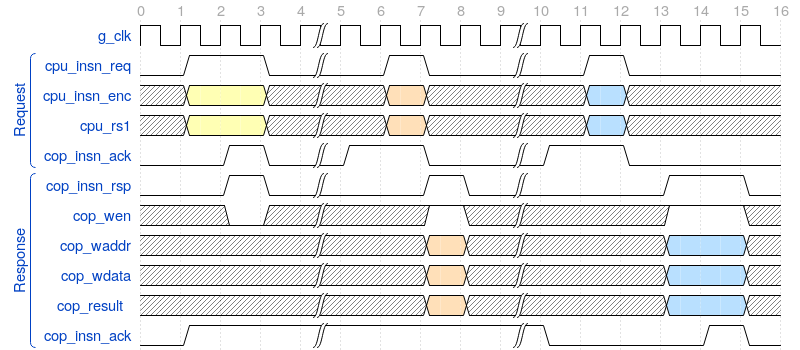
\includegraphics[width=\textwidth]{./diagrams/cpu-cop-if-1.png}
\caption{Simple instruction request, acknowledge, result with delays.
The first transaction shows an instruction request in cycle 1, followed
by the acknlowedgement and result in cycle 2.
The second shows that if {\tt cop\_insn\_ack} is set already, then
instructions can be accepted immediately and their result returned on the next
cycle.  The third shows how the request / acknowledge protocol handles
stalls.}
\end{figure}

\begin{figure}[h]
\caption{Back to back instruction requst, acknowledge, result.}
\end{figure}

\begin{figure}[h]
\caption{Multi-cycle instruction request, acknowledge, result.}
\end{figure}

\subsection{Memory Interface}


\section{COP Internal Micro-architecture}
\label{sec:cop-microarch}

\subsection{COP Register File}

\subsection{Packed Arithmetic Unit}

\subsection{Multi-precision Arithmetic Unit}

\subsection{Memory Unit}


\section{Integration Guide}
\label{sec:integration}


\section{Verification}
\label{sec:verification}


\printbibliography


\end{document}
